% eeprom-lib.tex
% i2c-eeprom library document.

\documentclass[11pt,a4paper]{article}

\usepackage{graphicx}
\usepackage{indentfirst}
\usepackage{verbatim}
%\usepackage{multirow}
%\usepackage{fancybox}
%\usepackage{endnotes}

\title{I2C EEPROM Library: AVR and AT24CXXX}
\author{sun\_ge@yahoo.cn}

\begin{document}

\maketitle

\begin{center}
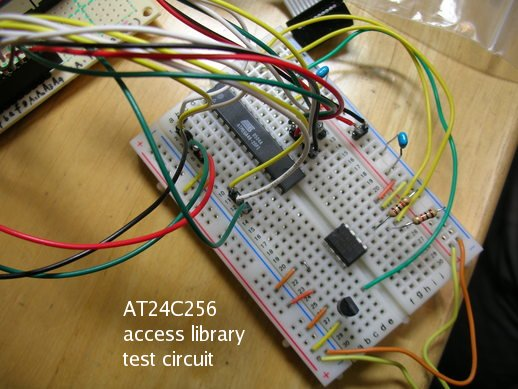
\includegraphics{i2c-eeprom.jpg}
\end{center}

\section{Project Origin}
AVR's I2C bus is simple, easy to use, and a lot of I2C devices can be attached together.
This I2C EEPROM access library was built for ATmega48 and AT24C128/256, may also
work for other microcontroller or I2C EEPROM with a little change.

\section{Hardware}

Please see {\em at24cxxx.h} for details.\\

\section{Source Code}
Source contains: at24cxxx.h, at24cxxx.c, i2c-eeprom-test.c and Makefile.\\
It can be compiled and installed by AVR GNU Tools Chain.

\subsection{I2C EEPROM Library Header: at24cxxx.h}
\verbatiminput{at24cxxx.h}

\subsection{I2C EEPROM Library: at24cxxx.c}
\verbatiminput{at24cxxx.c}

\subsection{Demo Program: i2c-eeprom-test.c}
\verbatiminput{i2c-eeprom-test.c}

\subsection{Makefile}
\verbatiminput{Makefile}

\end{document}

%%% Local Variables:
%%% coding: UTF-8
%%% mode: latex
%%% End:
